%
% gamma.tex -- Abschnitt über die Gamma-funktion
%
% (c) 2021 Prof Dr Andreas Müller, OST Ostschweizer Fachhochschule
%
\section{Die Gamma-Funktion
\label{buch:rekursion:section:gamma}}
\rhead{Gamma-Funktion}
Die Fakultät $x!$ kann rekursiv durch 
\[
	x! = x\cdot (x-1)! \qquad\text{und}\qquad 0!=1
\]
für alle natürlichen Zahlen $x\in\mathbb{N}$ definiert werden.
Äquivalent damit ist eine Funktion 
\begin{equation}
\Gamma(x+1) = x\Gamma(x)
\qquad\text{und}\qquad 
\Gamma(1)=1.
\label{buch:rekursion:eqn:gammadef}
\end{equation}
Kann man eine reelle oder komplexe Funktion finden, die die
Funktionalgleichung~\eqref{buch:rekursion:eqn:gammadef}
erfüllt und damit die Fakultät auf beliebige Argumente ausdehnt?

\subsection{Produktformel}
Die Fakultät $n!$ ist ein Produkt von $n$ Faktoren, es ist daher
natürlich zu versuchen, auch $x!$ als ein Produkt zu schreiben.
Allerdings kann es nicht möglich sein, dies mit einer endlichen
Anzahl von Faktoren zu machen, denn wenn $x$ grösser wird, muss auch
die Zahl der Faktoren grösser werden.
Mit jedem zusätzlichen Faktor ist ein Sprung der Werte zu erwarten.
Wir erwarten daher entweder ein unendliches Produkt oder einen
Ausdreck, bei dem die ``Anzahl'' $x$ der Faktoren im Exponenten
steht.
In diesem Abschnitt soll zunächst eine solcher Ausdruck gefunden
werden.
Dieser ist jedoch für die numerische Berechnung absolut ungeeignet,
so dass er später in ein unendliches Produkt umgeformt werden muss.

\subsubsection{Fakultät als Bruch}
Euler hat das Problem, die Fakultät auf beliebige reelle oder komplexe
Zahlen auszudehnen, wie folgt angepackt.
Zunächst hat er bemerkt, dass für ganzzahlige $x$ und natürliche $n$
\begin{align}
x! 
&=
1\cdot 2\cdot 3\cdot\ldots\cdot x
\notag
\\
&=
\frac{
1\cdot 2\cdot 3\cdot\ldots\cdot x\cdot (x+1) (x+2)\cdots(x+n)
}{
(x+1)(x+2)\cdots(x+n)
}
\notag
\\
&=
\frac{
1\cdot 2\cdot\ldots\cdot n\cdot(n+1)\cdot(n+2)\cdots(n+x)
}{
(x+1)(x+2)\cdots(x+n)
}
\notag
\\
&=
\frac{n! \cdot (n+1)(n+1)\cdots(n+x)}{(x+1)(x+2)\cdots(x+n)}
\label{buch:rekursion:gamma:eqn:fakultaet}
\end{align}
gilt.
Der Plan ist, dies so umzuformen, dass man für $x$ eine beliebige
komplexe Zahl einsetzen kann.

\subsubsection{Pochhammer-Symbol}
Die spezielle Form des Nenners und des zweiten Faktors im Zähler
von \eqref{buch:rekursion:gamma:eqn:fakultaet}
rechtfertigt die folgende Definition.

\begin{definition}[Pochhammer]
Für $a\in\mathbb{C}$ und $n\in\mathbb{N}$ heisst das Produkt
\[
(a)_n = a\cdot(a+1)\cdot(a+2)\cdots(a+n-1)
\]
das Pochhammer-Symbol oder die verschobene Fakultät.
\index{Pochhammer-Symbol}
\end{definition}

Die verschobene Fakultät $(a)_n$ hat also genau $n$ Faktoren, deren
erster $1$ ist.
Die gewöhnliche Fakultät hat $n$ Faktoren, deren erster $1$ ist, also
ist $n! = (1)_n$.

Der Ausdruck \eqref{buch:rekursion:gamma:eqn:fakultaet}
für $x!$ wird unter Verwendung des Pochhammer-Symbols zu
\begin{equation}
x! = \frac{n! (n+1)_x}{(x+1)_n}.
\label{buch:rekursion:gamma:eqn:produkt2}
\end{equation}
Leider ist dieser Ausdruck ebenfalls nicht auf beliebige $x$
verallgemeinerungsfähig, denn $(n)_x$ ist nur natürliche $x$ definiert.
Der Faktor $(n+1)_x$ enthält $x$ Faktoren beginnend bei $n$.
Für grosses $n$ sind diese Faktoren nahe beeinander, man sollte also
$(n+1)_x$ durch $n^x$ approximieren können.
Wir erweitern daher \eqref{buch:rekursion:gamma:eqn:produkt2} mit $n^x$
und erhalten
\begin{equation}
x!
=
\frac{n!\,n^x}{(x+1)_n}\cdot
\frac{(n+1)_x}{n^x}.
\label{buch:rekursion:gamma:eqn:produkt3}
\end{equation}
Der erste Faktor in diesem Ausdruck enthält jetzt nur noch Dinge,
die für beliebige $x\in\mathbb{C}$ definiert sind.

\subsubsection{Grenzwertdefinition}
Der zweite Bruch in \eqref{buch:rekursion:gamma:eqn:produkt3}
besteht aus Termen, die zwar nur für natürliches $x$ definiert sind,
wir vermuten aber, dass er für grosses $n$ gegen $1$ konvergiert.
Tatsächlich gilt
\[
\lim_{n\to\infty}
\frac{(n+1)_x}{n^x}
=
\lim_{n\to\infty}
\underbrace{\frac{n+1}{n}}_{\displaystyle\to 1}
\cdot
\underbrace{\frac{n+2}{n}}_{\displaystyle\to 1}
\cdot\ldots\cdot
\underbrace{\frac{n+x}{n}}_{\displaystyle\to 1}
=
1,
\]
da  $(n+x)/n=1+x/n\to 1$ für grosses $n$.
Dies würde die folgende Definition rechtfertigen.

\begin{definition}
\label{buch:rekursion:gamma:def:definition}
Die Gamma-Funktion $\Gamma(x)$ einer Zahl
$x\in\mathbb{C}\setminus\{0,-1,-2,-3,\dots\}$ ist der Grenzwert
\[
\Gamma(x) = \lim_{n\to\infty} \frac{n!\,n^{x-1}}{(x)_n}.
\] 
\end{definition}

\subsubsection{Rekursionsgleichung für $\Gamma(x)$}
Es ist aus der Herleitung klar, dass $\Gamma(n)=(n-1)!$ sein muss.
Wir sollten dies aber auch direkt aus der
Definition~\ref{buch:rekursion:gamma:def:definition} ableiten
können.
Dazu müssen wir nur überprüfen, ob $\Gamma(1)=0!=1$ ist und ob
die Rekursionsformel $\Gamma(n)=n\Gamma(n-1)$ gilt.

Den Wert $\Gamma(1)$ kann man direkt berechnen:
\[
\Gamma(1)
=
\lim_{n\to\infty} \frac{n!}{(1)_n}
=
\lim_{n\to\infty} \frac{n!}{n!}
=
1
\]
wegen $(1)_n=n!$.

Für die Rekursionsformel muss man den Grenzwert für $x$ und $x+1$
miteinander vergleichen.
Aus dem Term $(x+1)_n$ im Nenner muss man einen Term $(x)_n$ machen,
dies ist möglich, indem man mit $x$ erweitert:
\begin{align*}
\Gamma(x+1)
&=
\lim_{n\to\infty}\frac{n!\,n^x}{(x+1)_n}
=
x\lim_{n\to\infty}\frac{n!\,n^x}{x(x+1)_n}
=
x\lim_{n\to\infty}\frac{n!\,n^x}{(x)_{n+1}}.
\intertext{Wir müssen jetzt nur noch zeigen, dass der Grenzwert
auf der rechten Seite gegen $\Gamma(x)$ konvergiert,
in dessen Definition aber die Potenz $n^{x-1}$ vorkommt.
Wir müssen also einen Faktor $n$ los werden und gleichzeitig
aus $n$ überall $n+1$ machen, damit der Nenner wieder passt.
Dabei wird}
\Gamma(x+1)
&=
x\lim_{n\to\infty}
\frac{(n+1)!n^{x-1}}{(x)_{n+1}}
\cdot
\underbrace{\frac{n}{n+1}}_{\displaystyle\to 1}
\\
&=
x\lim_{n\to\infty}
\underbrace{\frac{(n+1)!(n+1)^{x-1}}{(x)_{n+1}}}_{\displaystyle\to\Gamma(x)}
\cdot
\frac{n^{x-1}}{(n+1)^{x-1}}
\\
&=
\Gamma(x)
\lim_{n\to\infty} \biggl(\frac{n}{n+1}\biggr)^{x-1}
=
\Gamma(x),
\end{align*}
Weil $n/(n+1)\to 1$ ist und die Funktion $z\mapsto z^{x-1}$ für alle
nach der Definition zulässigen Werte von $x$ eine stetige Funktion ist.

\subsubsection{Numerische Unzulänglichkeiten der Grenzwertdefinition}
Die Grenzwertdefinition~\ref{buch:rekursion:gamma:def:definition}
ist zwar zweifellos richtig, kann aber nicht für die numerische 
Berechnung der Gamma-Funktion verwendet werden.
Die Existenz des Grenzwertes verwendet, dass $x\ll n$ sein muss,
damit $(n+x)/n$ gegenüber $1$ vernachlässigt werden kann.
Die Grenzwertdefinition beginnt also erst, vernünftige Approximationen
von $\Gamma(x)$ zu geben, wenn $n$ viel grösser also $x$ ist.
Andererseits wächst $n!$ sehr schnell an, schon für $n=171$ ist
das Resultat grösser als was der \texttt{double}-Datentyp fassen kann.
Dies ist aber viel zu kleine, um gute Approximationen auch für kleine
Werte von $x$ zu geben.
So findet man zum Beispiel für $x=\frac12$ und $n=170$ mit Octave
\[
\frac{n!\,n^{x-1}}{(x)_n}
=
\frac{170!}{\sqrt{170}\cdot \frac12\cdot\frac32\cdot\ldots\cdot\frac{339}{2}}
=
\frac{7.2574\cdot10^{307}}{13.308\cdot 3.1381\cdot10^{305}}
=
1.7738.
\]
Andererseits werden wir später sehen, dass 
\[
\Gamma({\textstyle\frac12})
=
\sqrt{\pi}
=
1.772453850905516
\]
ist.
Die Approximation mit Hilfe der Grenzwertdefinition kann also
grundsätzlich nicht mehr als zwei korrekte Nachkommastellen liefern.

\subsubsection{Produktformel}
Ein möglicher Ausweg aus den numerischen Schwierigkeiten mit der
Grenzwertdefinition ist, den schnell wachsenden Faktor $n!$
in den Zähler zu bringen, so dass er der Konvergenz etwas nachhilft.
Wir berechnen daher den Kehrwert $1/\Gamma(x)$.

\begin{satz}
\label{buch:rekursion:gamma:satz:produktformel}
Der Kehrwert der Gamma-Funktion kann geschrieben werden als
\begin{equation}
\frac{1}{\Gamma(x)}
=
xe^{\gamma x}
\prod_{k=1}^\infty
\biggl(1+\frac{x}k\biggr)\,e^{-\frac{x}{k}},
\label{buch:rekursion:gamma:eqn:produktformel}
\end{equation}
wobei $\gamma$ die Euler-Mascheronische Konstante
\[
\gamma
=
\lim_{n\to\infty}
\biggl(\sum_{k=1}^n\frac{1}{k}-\log n\biggr)
\]
ist.
\end{satz}

\begin{proof}[Beweis]
Es sind zwei Dinge nachzuprüfen.
Zunächst muss nachgewiesen werden, dass das unendliche Produkt 
überhaupt konvergiert.
Wenn das gesichert ist, muss noch gezeigt werden, dass der Grenzwert
tatsächlich $1/\Gamma(x)$ ist.

Für die Konvergenz beachtet man, dass die Faktoren des Produkts 
die Form
\begin{align*}
\biggl(1+\frac{x}n\biggr)e^{-\frac{x}{n}}
&=
\biggl(1+\frac{x}n\biggr)
\biggl(1-\frac{x}{n}+\frac{x^2}{2n^2}-\frac{x^3}{3!n^3}+\dots\biggr)
\\
&=
1-\frac{x^2}{n^2} + 
\biggl(1+\frac{x}n\biggr)
\biggl(\frac{x^2}{2n^2}-\dots\biggr)
\\
&=
1-\frac{x^2}{n^2} + \frac{x^2}{2n^2} + O\bigl((\textstyle\frac{x}{n})^2\bigr)
\\
&=
1-\frac{x^2}{2n^2} + O\bigl((\textstyle\frac{x}{n})^3\bigr)
\end{align*}
haben.
Da die Reihe 
\[
\sum_{n=1}^\infty \frac{x^2}{n^2}
\]
konvergent ist, konvergiert auch das Produkt.
% XXX wir brauchen irgendwo das Konvergenzkriterium für ein Produkt

Um die Übereinstimmung der Produktformel mit $1/\Gamma(x)$ zu zeigen,
berechnen wir
\begin{align*}
\frac{1}{\Gamma(x)}
&=
\lim_{n\to\infty} 
\frac{(x)_n}{n!\,n^{x-1}}
=
\lim_{n\to\infty} 
\frac{x(x+1)(x+2)\cdots(x+n-1)}{1\cdot 2\cdot3\cdots (n-1)\cdot n\cdot n^{x-1}}
\\
&=
x
\lim_{n\to\infty} 
\frac{x+1}{1}
\cdot
\frac{x+2}{2}
\cdots
\frac{x+n-1}{n-1}
\cdot
n^{-x}
\\
&=
x
\lim_{n\to\infty}
\biggl(1+\frac{x}{1}\biggr)
\cdot
\biggl(1+\frac{x}{2}\biggr)
\cdots
\biggl(1+\frac{x}{n-1}\biggr)
\cdot
e^{-x\log n}
\\
&=
x
\prod_{k=1}^{n-1}
\biggl(1+\frac{x}{k}\biggr)
e^{-\frac{x}{k}}
e^{\frac{x}{k}}
e^{-x\log n}
\\
&=
x
\biggl(
\lim_{n\to\infty}
\prod_{k=1}^{n-1}
\biggl(1+\frac{x}{k}\biggr)
e^{-\frac{x}{k}}
\biggr)
\cdot
\biggl(
\lim_{n\to\infty}
e^{x\bigl(\sum_{k=1}^{n-1}\frac{1}{k} - \log n\bigr)}
\biggr)
\end{align*}
Der Klammerausdruck im Exponent des letzten Faktors auf der rechten Seite
konvergiert nach Definition der Euler-Mascheronischen Konstanten gegen
$\gamma$, somit folgt 
\[
\frac{1}{\Gamma(x)}
=
xe^{\gamma x}\prod_{k=1}^\infty \biggl(1+\frac{x}{k}\biggr)e^{-\frac{x}{k}},
\]
wie behauptet.
Damit ist Satz~\ref{buch:rekursion:gamma:satz:produktformel}
vollständig bewiesen.
\end{proof}

\begin{table}
\centering
\begin{tabular}{|>{$}c<{$}|>{$}c<{$}|>{$}c<{$}|}
\hline
k &  \Gamma(\frac12,n) & \Gamma(\frac12) - \Gamma(\frac12,n) \\
\hline
1 & 1.\underline{7}518166478 & -0.0206372031 \\
2 & 1.\underline{77}02543372 & -0.0021995137 \\
3 & 1.\underline{772}2324556 & -0.0002213953 \\
4 & 1.\underline{7724}316968 & -0.0000221541 \\
5 & 1.\underline{77245}16354 & -0.0000022156 \\
6 & 1.\underline{772453}6293 & -0.0000002216 \\
\hline
\end{tabular}
\caption{Werte $\Gamma(\frac12,n)$ von $\Gamma(\frac12)$ berechnet mit
$n=10^k$ Faktoren der
Produktformel~\eqref{buch:rekursion:gamma:eqn:produktformel}
und der zugehörige Fehler.
Die korrekten Nachkommastellen sind unterstrichen.
\label{buch:rekursion:gamma:gammatabelle}}
\end{table}

Um zu zeigen, dass die Produktform tatsächlich besser geeignet ist,
sind in der Tabelle~\ref{buch:rekursion:gamma:gammatabelle}
die Resultate der numerischen Rechnung  bis $n=1000000$ zusammengestellt.
Die Produktformel kann gute Werte von $\Gamma(x)$ auch für derart grosse
Werte von $n$ problemlos berechnen.

Der Fehler der numersichen Approximation ist von der Grössenordnung
$O(1/n)$ wie das auf Grund des verwendeten Konvergenzkriteriums
zu erwarten war.
Die Anzahl zu berücksichtigender Terme wächst daher exponentiall
mit der Anzahl gewünschter Stellen an, was für praktische Zwecke
zu langsam ist.
Für die numersiche Berechnung der Gamma-Funktion ist die Produktformel
daher im Allgemeinen nicht geeignet.

%
% Integralformel für die Gamma-Funktion
%
\subsection{Integralformel für die Gamma-Funktion}
Euler hat die folgende Integraldefinition der Gamma-Funktion gegeben.

\begin{definition}
\label{buch:rekursion:def:gamma}
Die Gamma-Funktion ist die Funktion 
\[
\Gamma
\colon
\{z\in\mathbb{C} \mid \operatorname{Re}z>0\}
\to \mathbb{C}
:
z
\mapsto
\Gamma(z) = \int_0^\infty t^{z-1}e^{-t}\,dt
\]
\end{definition}

Man beachte, dass das Integral für $x=0$ nicht definiert ist, eine
Potenzreihenentwicklung um einen Punkt $x_0$ auf der positiven reellen
Achse kann also höchstens den Konvergenzradius $\varrho=|x_0|$ haben.

\begin{figure}
\centering
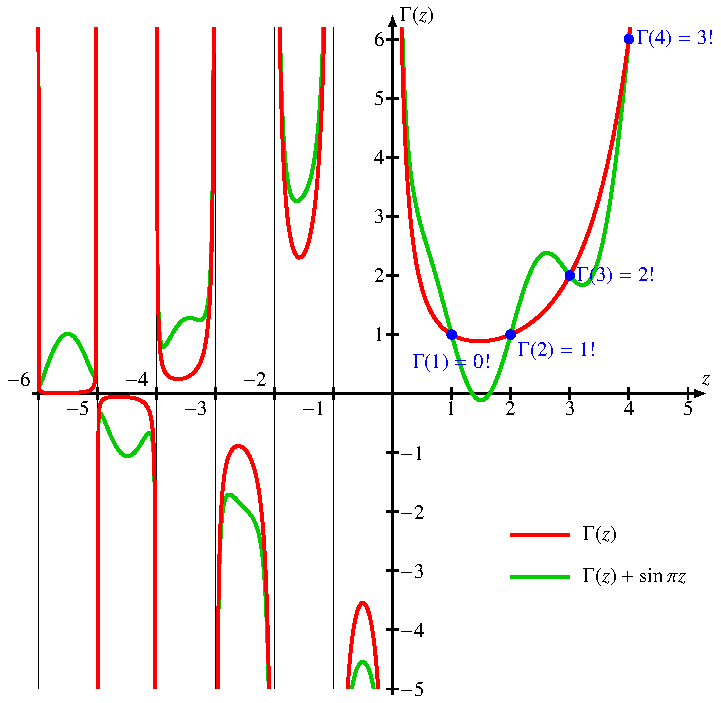
\includegraphics{chapters/040-rekursion/images/gammaplot.pdf}
\caption{Graph der Gamma-Funktion $z\mapsto\Gamma(z)$ und der alternativen
Funktion $\Gamma(z)+\sin(\pi z)$, die für ganzzahlige Argumente ebenfalls
die Werte der Fakultät annimmt.
\label{buch:rekursion:fig:gamma}}
\end{figure}

\subsubsection{Alternative Lösungen}
Die Funktion $\Gamma(z)$ ist nicht die einzige Funktion, die natürlichen
Zahlen die Werte $\Gamma(n+1) = n!$ der Fakultät annimmt.
Indem man eine beliebige Funktion $f(z)$ addiert, die auf alle
natürlichen Zahlen verschwindet, also $f(n)=0$ für $n\in\mathbb{N}$,
erhält man eine weitere Funktion, die auf natürlichen Zahlen
die Werte der Fakultät annimmt.
Ein Beispiel einer solchen Funktion ist
\begin{equation}
z\mapsto f(z)=\Gamma(z) + \sin \pi z,
\label{buch:rekursion:eqn:gammaalternative}
\end{equation}
die Funktion $f(z)=\sin\pi z$ verschwindet sogar auf allen ganzen
Zahlen.

In Abbildung~\ref{buch:rekursion:fig:gamma} ist die Gamma-Funktion
in rot geplotet, die Funktion~\eqref{buch:rekursion:eqn:gammaalternative}
in grün.
Die Punkte $(n,(n-1)!)$ sind in blau bezeichnet, sie sind beiden Graphen
gemeinsam.

\subsubsection{Pol erster Ordnung bei $z=0$}
Wir haben zu prüfen, dass sowohl der Wert $\Gamma(1)$ korrekt ist als
auch die Rekursionsformel~\eqref{buch:rekursion:eqn:gammadef} gilt.
Der Wert für $z=1$ ist
\begin{align*}
\Gamma(1)
&=
\int_0^\infty t^{1-1}e^{-t}\,dt
=
\left[ -e^{-t} \right]_0^\infty
=
1.
\end{align*}
Für die Rekursionsformel kann mit Hilfe von partieller Integration
bekommen:
\begin{align*}
\Gamma(z+1)
&=
\int_0^\infty t^{z+1-1}e^{-t}\,dt
=
\biggl[-t^{z}e^{-t}\biggr]_0^\infty
+
\int_0^\infty z t^{z-1}e^{-t}\,dt
\\
&=
z
\int_0^\infty
t^{z-1}e^{-t}\,dt
=
z \Gamma(z).
\end{align*}

Für $0<z<\varepsilon$ für eine $\varepsilon >0$ folgt aus der 
Funktionalgleichung
\[
\Gamma(z) = \frac{\Gamma(1+z)}{z}.
\]
Da $\Gamma(1)=1$ ist und $\Gamma$ eine in einer
Umgebung von $1$ stetige Funktion ist, kann sie in der Form
\(
\Gamma(1+z)=\Gamma(1) + zf(z)
\)
schreiben, wobei  $f(z)$ eine differenzierbare Funktion ist mit
$f'(1)=\Gamma'(1)$.
Daraus ergibt sich für $\Gamma(z)$ der Ausdruck
\[
\Gamma(z) = \frac{\Gamma(1)}{z} + f(z) = \frac{1}{z} + f(z).
\]
Die Gamma-Funktion hat daher and er Stelle $z=0$ einen Pol erster Ordnung.

\subsubsection{Ausdehnung auf $\operatorname{Re}z<0$}
Die Integralformel konvergiert nicht für $\operatorname{Re}z\le 0$.
Durch analytische Fortsetzung, wie sie im
Abschnitt~\ref{buch:funktionentheorie:section:fortsetzung}
beschrieben wird, kann die Funktion auf ganz $\mathbb{C}$ ausgedehnt
werden, mit Ausnahme einzelner Pole.
Die Funktionalgleichung gilt natürlich für alle $z\in\mathbb{C}$,
für die $\Gamma(z)$ definiert ist.
In einer Umgebung von $z=-n$ gilt
\[
\Gamma(z)
=
\frac{\Gamma(z+1)}{z}
=
\frac{\Gamma(z+2)}{z(z+1)}
=
\frac{\Gamma(z+3)}{z(z+1)(z+2)}
=
\dots
=
\frac{\Gamma(z+n)}{z(z+1)(z+2)\cdots(z+n-1)}
\]
Keiner der Faktoren im Nenner verschwindet in der Nähe von $z=-n$, der
Zähler hat aber einen Pol erster Ordnung an dieser Stelle.
Daher hat auch der Quotient einen Pol erster Ordnung.
Abbildung~\ref{buch:rekursion:fig:gamma} zeigt die Pole bei den
nicht negativen ganzen Zahlen.

\subsubsection{Numerische Berechnung}
\begin{table}
\centering
\begin{tabular}{|>{$}c<{$}|>{$}c<{$}>{$}c<{$}|}
\hline
k & y(10^k) & y(10^k) - \Gamma(\frac{5}{2}) \\
\hline
1 & 0.0000000000 & -0.9027452930 \\
2 & 0.3319129461 & -0.5708323468 \\
3 & 0.\underline{902}5209490 & -0.0002243440 \\
4 & 0.\underline{902745}1207 & -0.0000001723 \\
5 & 0.\underline{902745}0962 & -0.0000001968 \\
6 & 0.\underline{902745}0962 & -0.0000001968 \\
\hline
\end{tabular}
\caption{Resultate der Berechnung von $\Gamma(\frac{5}{2})$ mit Hilfe
der Differentialgleichung \eqref{buch:rekursion:gamma:eqn:gammadgl}.
Die korrekten Stellen sind unterstrichen.
Es sind immerhin sechs korrekte Stellen gefunden, wobei nur 337
Auswertungen des Integranden notwendig waren.
\label{buch:rekursion:gamma:table:gammaintegral}}
\end{table}
Im Prinzip könnte die Integraldefinition der numerischen Berechnung
entgegenkommen.
Um diese Hypothese zu prüfen, berechnen wir das Integral für
$z=\frac52$ mit Hilfe der äquivalenten Differentialgleichungen
\begin{equation}
\dot{y}(t) = t^{z-1}e^{-t}
\qquad\text{mit Anfangsbedingung $y(0)=0$}.
\label{buch:rekursion:gamma:eqn:gammadgl}
\end{equation}
Der gesuchte Wert ist der Grenzwert $\lim_{t\to\infty} y(t)$.
In der Tabelle~\ref{buch:rekursion:gamma:table:gammaintegral}
sind die Werte von $y(10^k)$ sowie die Differenzen 
$y(10^k) - \Gamma(\frac{5}{2})$ zusammengefasst.
Die Genauigkeit erreicht sechs korrekte Nachkommastellen mit nur
337 Auswertungen des Integranden.

%
% Beta-Integrale
%
\subsection{Die Beta-Funktion}

\begin{definition}
\label{buch:rekursion:gamma:def:beta-funktion}
Das Beta-Integral ist das Integral
\[
B(x,y)
=
\int_0^1 t^{x-1} (1-t)^{y-1}\,dt
\]
für $\operatorname{Re}x>0$, $\operatorname{Re}y>0$.
\end{definition}

Aus der Definition kann man sofort ablesen, dass $B(x,y)=B(y,x)$.
Für $y=1$ folgt ausserdem
\[
B(x,1) = \int_0^1 t^{x-1}\,dt = \biggl[ \frac{t^x}{x}\biggr]_0^1 = \frac{1}{x}.
\]
Speziell gilt $B(1,1)=1$.

\subsubsection{Rekursionsformeln für das Beta-Integral}
Aus der Definition folgt direkt
\begin{align*}
B(x,y+1)
&=
\int_0^1 t^{x-1} (1-t)^{y+1-1}\,dt
=
\int_0^1 (1-t) t^{x-1} (1-t)^{y-1}\,dt
\\
&=
\int_0^1 t^{x-1} (1-t)^{y-1}\,dt
-
\int_0^1 t^{x} (1-t)^{y-1}\,dt
\\
&=
B(x,y) - B(x+1,y)
\end{align*}
oder
\begin{equation}
B(x+1,y) = B(x,y) - B(x,y+1).
\label{buch:rekursion:gamma:betarek1}
\end{equation}
%
%XXX Vergleich mit der Rekursionsformel für Binomialkoeffizienten
%
Durch partielle Integration kann man eine weitere Rekursionsformel finden.
Dazu berechnet man
\begin{align}
B(x,y+1)
&=
\int_0^1 t^{x-1}(1-t)^{y}\,dt
\notag
\\
&=
\biggl[\frac{t^x}x(1-t)^y\biggr]_0^1
+
\frac{y}x \int_0^1 t^x(1-t)^{y-1}\,dt
\notag
\\
&=
 \frac{y}x B(x+1,y).
\label{buch:rekursion:gamma:betarek2}
\end{align}
Durch Gleichsetzen
\eqref{buch:rekursion:gamma:betarek1}
und
\eqref{buch:rekursion:gamma:betarek2}
entsteht die Rekursionsformel
\[
B(x,y)-B(x,y+1)
=
B(x+1,y)
=
\frac{x}{y}B(x,y+1)
\]
oder
\begin{equation}
B(x,y)
=
\frac{x+y}{y}B(x,y+1).
\label{buch:rekursion:gamma:betarek3}
\end{equation}

\subsubsection{Beta-Funktion und Gamma-Funktion}
Die Rekursionsbeziehung~\eqref{buch:rekursion:gamma:betarek3}
kann jetzt dazu verwendet werden, eine Darstellung der Beta-Funktion
durch die Gamma-Funktion zu finden.
Durch $n$-fache Anwendung von \eqref{buch:rekursion:gamma:betarek3}
ergibt sich zunächst
\begin{align*}
B(x,y)
&=
\frac{x+y}{y}
B(x,y+1)
=
\frac{x+y}{y}
\frac{x+y+1}{y+1}
B(x,y+2)
\\
&=
\frac{x+y}{y}
\frac{x+y+1}{y+1}
\cdot
\ldots
\cdot
\frac{x+y+n-1}{y+n-1}
B(x,y+n)
=
\frac{(x+y)_n}{(y)_n}
B(x,y+n)
\intertext{Die Beta-Funktion auf der rechten Seite kann als Integral
geschrieben werden:}
&=
\frac{(x+y)_n}{(y)_n}
\int_0^1 t^{x-1}(1-t)^{y+n-1}\,dt.
\intertext{Wir streben an, mit dem Grenzübergang $n\to\infty$ aus den
Pochhammer-Symbolen Gamma-Funktionen zu machen, dazu müssen gemäss
Definition~\ref{buch:rekursion:gamma:def:definition} weitere Faktoren
$1/(n!\,n^{x-1})$ vorhanden sein.
Wir erweitern geeignet und nehmen die übrig bleibenden Faktoren in
das Integral.
So ergibt sich}
&=
\frac{(x+y)_n}{n!\, n^{x+y-1}}
\frac{n!\,n^{y-1}}{(y)_n}
\int_0^1 n^{x} t^{x-1}(1-t)^{y+n-1}\,dt.
\intertext{Mit der Substition $s/n=t$ wird das Integral zu einem Integral
über das Interval $[0,n]$}
&=
\frac{(x+y)_n}{n!\, n^{x+y-1}}
\frac{n!\,n^{y-1}}{(y)_n}
\int_0^n
n^{x}
\biggl(\frac{s}{n}\biggr)^{x-1}
\biggl(1-\frac{s}{n}\biggr)^{y+n-1}
\,\frac{ds}{n}.
\\
&=
\frac{(x+y)_n}{n!\, n^{x+y-1}}
\frac{n!\,n^{y-1}}{(y)_n}
\int_0^n
n^{x-1}
\biggl(\frac{s}{n}\biggr)^{x-1}
\biggl(1-\frac{s}{n}\biggr)^{y+n-1}
\,ds.
\intertext{Beim Grenzübergang $n\to\infty$ wird daraus}
&=
\underbrace{\frac{(x+y)_n}{n!\, n^{x+y-1}}}_{\displaystyle \to 1/\Gamma(x+y)}
\underbrace{\frac{n!\,n^{y-1}}{(y)_n}}_{\displaystyle\to \Gamma(y)}
\int_0^n
s^{x-1}
\underbrace{\biggl(1-\frac{s}{n}\biggr)^{n}}_{\displaystyle\to e^{-s}}
\underbrace{\biggl(1-\frac{s}{n}\biggr)^{y-1}}_{\displaystyle\to 1}
\,ds.
\\
&\to \frac{\Gamma(y)}{\Gamma(x+y)} \int_0^\infty s^{x-1}e^{-s}\,ds
=
\frac{\Gamma(y)\Gamma(x)}{\Gamma(x+y)}.
\end{align*}

\begin{satz}
Die Beta-Funktion kann aus der Gamma-Funktion nach
\begin{equation}
B(x,y) = \frac{\Gamma(x)\Gamma(y)}{\Gamma(x+y)}
\label{buch:rekursion:gamma:betagamma}
\end{equation}
berechnet werden.
\end{satz}

\subsubsection{Der Wert von $\Gamma(\frac12)$?}
Als Anwendung der Formel~\eqref{buch:rekursion:gamma:betagamma}
untersuchen wir den Fall $y=1-x$.
In diesem Fall wird der Nenner zu $\Gamma(x+1-x)=\Gamma(1)=1$ und damit
\begin{equation}
\Gamma(x)\Gamma(1-x)
=
B(x,1-x) 
=
\int_0^1 t^{x-1}(1-t)^{-x}\,dt.
\label{buch:rekursion:gamma:spiegelung-betaintegral}
\end{equation}
Sofern man in der Lage ist, das Integral auf der rechten Seite von
\eqref{buch:rekursion:gamma:spiegelung-betaintegral} auszuwerten,
kann man eine einfache Beziehung zwischen zwei Werten der Gamma-Funktion
an Stellen, die durch eine Spiegelung an der Geraden
$\operatorname{Re}x=\frac12$ auseinander hervorgehen.
Für $x=\frac12$ wird der Ausdruck besonders einfach:
\[
\Gamma({\textstyle\frac12})^2
=
\int_0^1 t^{\frac12}(1-t)^{-\frac12}\,dt
=
\int_0^1 \sqrt{\frac{t}{1-t}}\,dt.
\]
Mit der Substition $t=\sin^2 s$ wird daraus
\[
\int_0^{\frac{\pi}2}
\sqrt{\frac{\sin^2s}{1-\sin^2s}}
2\sin s\cos s
\,ds
=
2
\int_0^{\frac{\pi}2}
\sin^2 s\,ds
=
2
\int_0^{\frac{\pi}2}
\frac{1-\cos 2s}{2}\,ds
=
\frac{\pi}2-\int_0^{\frac{\pi}2}\cos 2s\,ds,
\]
wobei wir $dt = 2\sin s\cos s\,ds$ verwendet haben.
Da $\cos 2s$ eine im Intervall $[0,\frac{\pi}2]$ bezüglich
des Punktes $\frac{\pi}4$ ungerade Funktion ist, verschwindet
das zweite Integral.
Somit folgt
\begin{equation}
\Gamma({\textstyle\frac12})^2 = \frac{\pi}{2}
\qquad\Rightarrow\qquad
\Gamma({\textstyle\frac12}) = \sqrt{\frac{\pi}{2}}.
\label{buch:rekursion:gamma:gamma12}
\end{equation}
Matt Parker hat auf seinem Youtube-Kanal {\em Stand-up Maths} dieses Resultat
sogar zum Titel eines Videos\footnote{\url{https://youtu.be/dGnIJFzkLI4}}
gemacht:
{\em What is the factorial of $-\nicefrac{1}{2}$?}
Die Antwort ist natürlich nur möglich, indem man
$(-\frac12)!$ als Wert
\[
(-{\textstyle\frac12})!
=
\Gamma(-{\textstyle\frac12}+1)
=
\Gamma({\textstyle\frac12})
=
\sqrt{\frac{\pi}2}
\]
der Gamma-Funktion interpretiert.

\subsubsection{Alternative Parametrisierungen}
Die Substitution $t=\sin^2 s$ hat im vorangegangenen Abschnitt
ermöglicht, $\Gamma(\frac12)$ zu ermitteln.
Die Substition erlaubt aber auch, das Beta-Integral in eine alternative
Form zu bringen.
Aus der Definition~\ref{buch:rekursion:gamma:def:beta-funktion}
wird damit
\begin{align*}
B(x,y)
&=
\int_0^1 t^{x-1} (1-t)^{y-1}\,dt
\\
&=
2
\int_0^{\frac{\pi}2} \sin^{2(x-1)} s\cdot (1-\sin^2 s)^{y-1}
\cdot \sin s\cos s\,ds
\\
&=
2
\int_0^{\frac{\pi}2} \sin^{2x-1}s \cos^{2y-1} s\,ds.
\intertext{Unter Verwendung der Formel~\eqref{buch:rekursion:gamma:betagamma},
die die Beta-Funktion durch Gamma-Funktionen auszudrücken erlaubt, findet
man die Formel}
\int_0^{\frac{\pi}2} \sin^{2x-1}s \cos^{2y-1} s\,ds
&=
\frac{\Gamma(x)\Gamma(y)}{2\Gamma(x+y)}
\end{align*}
für ein bestimmtes Integral von Potenzen von Sinus- und Kosinus-Funktionen.

Die alternative Substitution $t = s/(s+1)$ verwandelt das Beta-Integral
$B(x,y)$ in ein Integral über die positive Halbachse ab:
\begin{align}
B(x,y)
&=
\int_0^1 t^{x-1}(1-t)^{y-1}\,dt
\notag
\\
&=
\int_0^\infty
\frac{s^{x-1}}{(s+1)^{x-1}}
\frac{1}{(s+1)^{y-1}}
\frac{ds}{(s+1)^2}
\notag
\\
&=
\int_0^\infty
\frac{s^{x-1}}{(s+1)^{x+y}}\,ds,
\label{buch:rekursion:gamma:beta:sinf}
\end{align}
wobei wir
\[
\frac{dt}{ds}
=
\frac{d}{ds}
\frac{s}{s+1}
=
\frac{(s+1)-s}{(s+1)^2}
=
\frac{1}{(s+1)^2}
\]
verwendet haben.
Diese Darstellung des Beta-Integrals wird später
% XXX Ort ergänzen
dazu verwendet, die Spiegelungsformel für die Gamma-Funktion
herzuleiten.

Eine weitere mögliche Parametrisierung verwendet $t = (1+s)/2$
mit $dt=\frac12 ds$.
Damit wird das Beta-Integral
\begin{equation}
B(x,y)
=
\int_0^1 t^{x-1}(1-t)^{y-1}\,dt
=
\frac12
\int_{-1}^1
\biggl(\frac{1+s}2\biggr)^{x-1}
\biggl(\frac{1-s}2\biggr)^{y-1}
\,ds
=
2^{1-x-y}
\int_{-1}^1
(1+s)^{x-1}(1-s)^{y-1}
\,ds.
\label{buch:rekursion:gamma:beta:symm}
\end{equation}

\subsubsection{Die Verdoppelungsformel von Legendre}
Die trigonometrische Substitution kann dazu verwendet werden, die
Legendresche Verdoppelungsformel für die Gamma-Funktion herzuleiten.

\begin{satz}[Legendre]
\[
\Gamma(x)\Gamma(x+{\textstyle\frac12})
=
2^{1-2x}\sqrt{\pi}
\Gamma(2x)
\]
\end{satz}

\begin{proof}[Beweis]
Der Wert $\Gamma(2x)$ entsteht, wenn man $B(x,x)$ mit Hilfe der
Gamma-Funktion als
\[
B(x,x)
=
\frac{\Gamma(x)^2}{\Gamma(2x)}
\]
schreibt.
Das Ziel ist, $B(x,x)$ auf einem alternativen Weg zu berechnen.

Mit Hilfe von \eqref{buch:rekursion:gamma:beta:symm}
kann man das Beta-Integral zu
\begin{align*}
B(x,x)
&=
2^{1-2x}
\int_{-1}^1
(1+s)^{x-1}(1-s)^{x-1}
\,ds
=
2^{1-2x}
\int_{-1}^1(1-s^2)^{x-1}\,ds
\end{align*}
vereinfachen.
Der Integrand ist gerade, es folgt
\[
B(x,x)
=
2^{1-2x}
\cdot 2
\int_0^1(1-s^2)^{x-1}\,ds.
\]
Das Integral kann mit der Substitution $s^2=t$ wieder in die Form
eines Beta-Integrals gebracht werden:
\begin{align*}
2\int_0^1(1-s^2)^{x-1}\,ds
&=
\int_0^1 (1-t)^{x-1} \,\frac{dt}{\sqrt{t}}
=
\int_0^1 t^{\frac12-1}(1-t)^{x-1}\,dt
=
B({\textstyle\frac12},x).
\end{align*}
In der Substitution haben wir $2s\,ds = dt$ oder $2\,ds = dt/\sqrt{t}$
verwendet.
Das letzte Beta-Integral kann man nun wieder mit Gamma-Funktionen
schreiben, nämlich als
\[
B({\textstyle\frac12},x)
=
\frac{\Gamma({\textstyle\frac12})\Gamma(x)}{\Gamma(x+{\textstyle\frac12})}.
\]
Setzt man alles zusammen, erhält man jetzt
\begin{align*}
\frac{\Gamma(x)^2}{\Gamma(2x)}
&=
\frac1{2^{2x-1}}
\frac{\Gamma({\textstyle\frac12})\Gamma(x)}{\Gamma(x+{\textstyle\frac12})}
\\
\Rightarrow\qquad
\Gamma(x)\Gamma(x+{\textstyle\frac12})
&=
2^{1-2x}
\Gamma({\textstyle\frac12})\Gamma(2x)
=
2^{1-2x}\sqrt{\pi}\Gamma(2x),
\end{align*}
wobei wir den bekannten Wert $\Gamma(\frac12)=\sqrt{\pi}$ verwendet haben.
\end{proof}

Setzt man $x=\frac12$ in die Verdoppelungsformel ein, erhält man
\[
\Gamma({\textstyle\frac12})\Gamma(1) = 2^{1-2\frac12}\sqrt{\pi}\Gamma(1)
\qquad\Rightarrow\qquad
\Gamma({\textstyle\frac12}) = \sqrt{\pi},
\]
in Übereinstimmung mit dem bereits bekannten Wert.

\subsubsection{Beta-Funktion und Binomialkoeffizienten}
Die Binomialkoeffizienten können mit Hilfe der Fakultät als
\begin{equation}
\binom{n}{k}
=
\frac{n!}{(n-k)!\,k!}
=
\frac{\Gamma(n-1)}{\Gamma(n-k-1)\Gamma(k-1)}
=
\frac{(n-2)\Gamma(n-2)}{\Gamma(n-k-1)\Gamma(k-1)}
=
\frac{n-2}{B(n-k-1,k-1)}
\label{buch:rekursion:gamma:binombeta}
\end{equation}
geschrieben werden.
Die Rekursionsbeziehung
\[
\binom{n+1}{k} = \binom{n}{k-1} + \binom{n}{k}
\]
der Binomialkoeffizienten erzeugt das vertraute Pascal-Dreieck,
die Formel \eqref{buch:rekursion:gamma:binombeta} für die
Binomialkoeffizienten macht daraus
\[
\frac{n-1}{B(n-k,k-1)}
=
\frac{n-2}{B(n-k,k-2)}
+
\frac{n-2}{B(n-k-1,k-1)},
\]
die für ganzzahlige Argumente gilt.
Wir wollen nachrechnen, dass dies für beliebige Argumente gilt.
\begin{align*}
\frac{(n-1)\Gamma(n-1)}{\Gamma(n-k)\Gamma(k-1)}
&=
\frac{(n-2)\Gamma(n-2)}{\Gamma(n-k)\Gamma(k-2)}
+
\frac{(n-2)\Gamma(n-2)}{\Gamma(n-k-1)\Gamma(k-1)}
\\
\frac{\Gamma(n)}{\Gamma(n-k)\Gamma(k-1)}
&=
\frac{\Gamma(n-1)}{\Gamma(n-k)\Gamma(k-2)}
+
\frac{\Gamma(n-1)}{\Gamma(n-k-1)\Gamma(k-1)}
\intertext{Durch Zusammenfassen der Faktoren im Zähler mit Hilfe
der Rekursionsformel für die Gamma-Funktion und Multiplizieren
mit dem gemeinsamen Nenner
$\Gamma(n-k)\Gamma(k-1)=(n-k-1)\Gamma(n-k-1)(k-2)\Gamma(k-2)$ wird daraus}
\Gamma(n)
&=
(k-2)
\Gamma(n-1)
+
(n-k-1)
\Gamma(n-1)
\intertext{Indem wir die Rekursionsformel für die Gamma-Funktion auf
die rechte Seite anwenden können wir erreichen, dass in allen Termen
ein Faktor
$\Gamma(n-1)$ auftritt:}
(n-1)\Gamma(n-1)
&=
(k-2)\Gamma(n-1)
+
(n+k-1)\Gamma(n-1)
\\
n-1
&=
k-2
+
n-k-1
\end{align*}


%
%
%

